\section{System identification}
\label{cap:system_identification}

In order to identify parameters $P_1 \hdots P_6$, introduced in chapter \ref{chap:uav_dynamics}, a test flight needed to be made. There are several methods of system identification for both time and frequency domain. Despite theirs advantages, one have to excite system poles and zeros in a way that could lead to damage of the system and its surroundings. In case of highly unstable UAV, testing by a step response or frequency response mostly unwanted. Instead the model can be fitted on arbitrary data using a mathematical optimization approach. The test flight, which was conducted by a human operator, consisted mainly of a hover above one place with small oscillations in all axis. All data used for following identification were gathered from an onboard \textbf{px4flow} optical flow sensor (inc. ultrasonic rangefinder). They were received and logged in constant rate of $88\jed{Hz}$ and coupled with appropriate control action of the operator. Since all searched parameters are part of a first order system, we can write down its discrete differential equation

\begin{equation}
q[n+1] = P_Aq[n] + P_Bu[n]
\end{equation}

where $P_A$, $P_B$ are desired constants of the transfer function. Supposing this is the correct description, all sensors are perfect and there are no other effects on the system, this equation should hold for all measured samples. When considering all samples, the set of equations can be written as follows

\begin{equation}
\textbf{B} = \textbf{A}\textbf{P}
\label{eq:bap}
\end{equation}

where \textbf{A} is the main matrix of the set, \textbf{B} is the left side of the equation and \textbf{P} is the vector of parameters we are looking for.

\begin{equation}
\textbf{A} = \begin{bmatrix}
q[1] & u[1] \\
q[2] & u[2] \\
\vdots & \vdots \\
q[m-1] & u[m-1] \\
\end{bmatrix},
\textbf{B} = \begin{bmatrix}
q[2] \\
q[3] \\
\vdots\\
q[m]
\end{bmatrix},
\textbf{P} = \begin{bmatrix}
P_A \\
P_B
\end{bmatrix}
\end{equation}

Due to the fact that the system description does not cover all phenomena and the measured data are noisy, the equation (\ref{eq:bap}) does not need to hold. But we can still estimate values of \textbf{P} in a way that $\norm{\textbf{AP-B}}_2^2$ is minimal. To provide a good chance of estimating all parameters well, such data should be supplied that the set of equations is overdetermined. The solution is then optimal in terms of least squares of \textbf{r}, where $\textbf{r} = \textbf{AP-B}$ is a vector of residuals of the equation system. This optimization problem can be solved e.g. manually using QR decomposition or using Matlab's '\textit{\textbackslash}' operator.

\subsection{Identifying Attitude axis}

There are four parameters, $P_1$, $P_2$ for \texttt{x} axis and $P_3$, $P_4$ for \texttt{y} axis. Assuming the system is decoupled and the low-level stabilization drive both subsystems identically\footnote{Further experiments show that both axis can be driven by the same controller utilizing a single model.} we can identify a model using only one of them. Following experiment was conducted using a manually controlled UAV equipped with a px4flow optical flow sensor. Data seen in fig. \ref{fig:iden1} are both unfiltered and captured onboard using a dedicated logging device. One could ask what are the units of the input signal. Values shown in the plot are fundamentally a time difference from a mean PPM signal pulse, measured using a hardware timer. They are directly proportional to the desired attitude angle of the UAV.

\begin{figure}[h!]
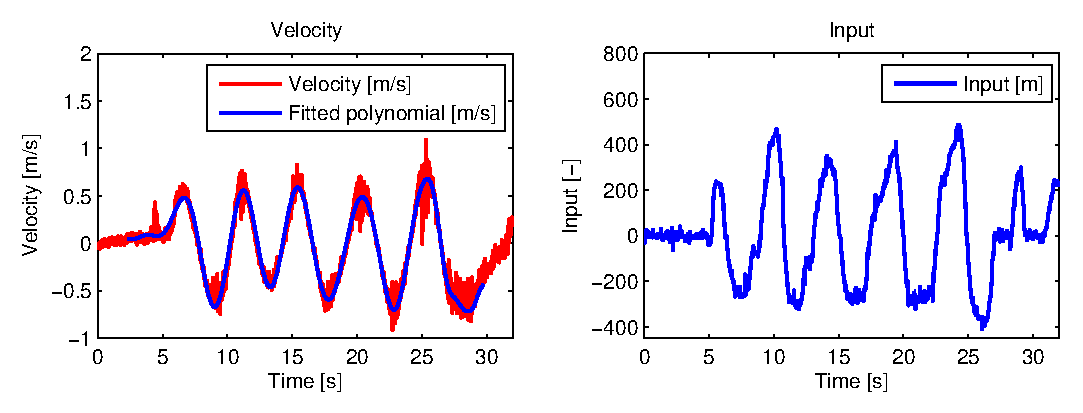
\includegraphics[width=1\textwidth]{fig/iden1.eps} 
\caption{Identification data - attitude}
\label{fig:iden1}
\end{figure}

To identify a first order transfer function from the input to the acceleration, one have to derive the velocity signal. Due to its large noise component, differentiating it discreetly was found impractical. Instead fitting a smooth function leads to computing the derivation analytically. The polynomial function was chosen to fit the data since it can be easily derived and can fit them well. Using the approach described above, constants $P_1$ and $P_2$ were obtained.

\begin{equation}
P_1 = 0.9799, P_2 = 5.0719 \times 10^{-5} 
\label{eq:constants1}
\end{equation}

Having these constants, the attitude system can be completed with particular values. 

\begin{equation}
\begin{split}
\mathbf{A}_{x, y} = \begin{bmatrix}
1 & 0.0114 & 0 \\
0 & 1 & 0.0114 \\
0 & 0 & 0.9799
\end{bmatrix}, \mathbf{B}_{x, y} = \begin{bmatrix}
0\\
0\\
5.0719 \times 10^{-5}
\end{bmatrix}
\end{split}
\end{equation}

The system can be further tested by estimating all states in open-loop from the measured input. We can evaluate its performance empirically by comparing estimates with measured data.

\begin{figure}[h!]
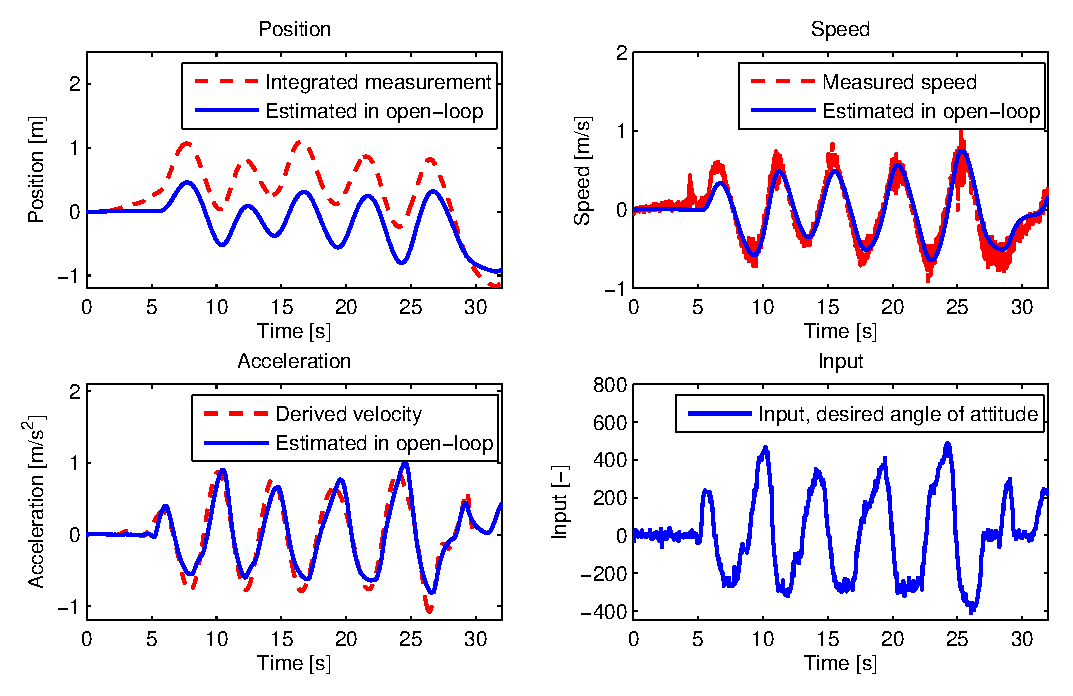
\includegraphics[width=1\textwidth]{fig/iden2.eps} 
\caption{Identification - open loop estimation}
\label{fig:iden2}
\end{figure}

As it can be seen in fig. \ref{fig:iden2} states estimated in open-loop are tracking the genuine values without much error. Some drift can be seen in the position, after the second integrator.